\section{Image Filtering}
\label{image_filtering}

In this section, we will 
be talking about image filtering through cross correlation and
convolution operations. We will also discuss some of the common uses for these operations and relate them to the self-driving task. 

\subsection{Why Do We Need Image Filtering?}
First, let us begin with the motivation on why we
would use image filtering. The image formation process is susceptible to lots of
different noise sources. An example is shown in Figure \ref{camera_man_1}.

\begin{figure}[!htb]
\begin{center}
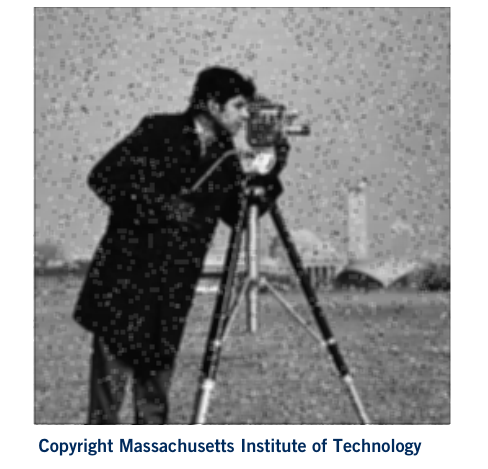
\includegraphics[scale=0.380]{img/visual_perception/camera_man_1.jpeg}
\end{center}
\caption{Example of a noise image.}
\label{camera_man_1}
\end{figure}

This is a very famous photo created at MIT that is used for testing
computer vision algorithms. Now let us add salt and
pepper noise to this image, by randomly turning some of its pixels white
and others black. How can we retrieve a reasonable visual appearance of the original image
from such a noisy one? Image filtering is as simple and efficient method
to eliminate noise. Moreover, depending on the filter, a variety of operations can be performed on images in
an efficient manner. But first, let us see how image filtering helps reduce salt and pepper noise as
a motivating example. 

\subsection{Reduce Image Noise}

If we look at the image array, we noticed that salt and pepper noise usually results in
outlier pixels, low-value pixels in a high-value neighborhood or high-value pixels in a low-value neighborhood, see Figure \ref{camera_man_2}. 

\begin{figure}[!htb]
\begin{center}
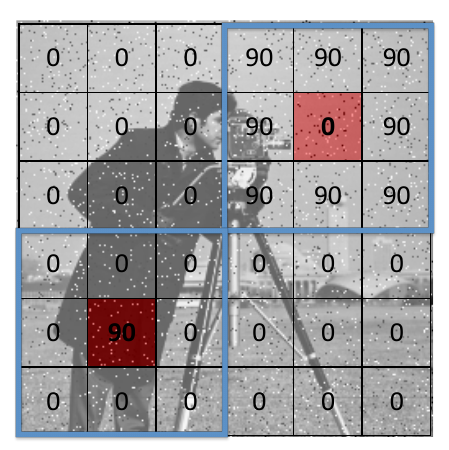
\includegraphics[scale=0.380]{img/visual_perception/camera_man_2.jpeg}
\end{center}
\caption{Schematic of outlier pixels.}
\label{camera_man_2}
\end{figure}

One idea to reduce this noise is to compute the mean of
the whole neighborhood, and replace the outlier pixel
with this mean value. Let us define $G$ as the output
of our filter operation. The equation of the mean can
be described in terms of $k$, $u$ and $v$ as shown in equation.

\begin{equation}
G(u,v) = \frac{1}{(2k+1)^2} \sum_{i=-k}^{k}\sum_{j=-k}^{k} I[u-i, v-j]
\label{simple_filter_equation}
\end{equation} 


Here, $2k+1$ is the filter size. In this case, the size of
our neighborhood which is three leads to a $k$
that is equal to one. $u$ and $v$ are the center pixel
image coordinates. Computing the mean
results in 80 for the top neighborhood and
10 for the bottom one. The final step is to
replace the center pixel of each of those neighborhoods
by the corresponding mean. The application of the so called mean filter results in

\begin{figure}[!htb]
\begin{center}
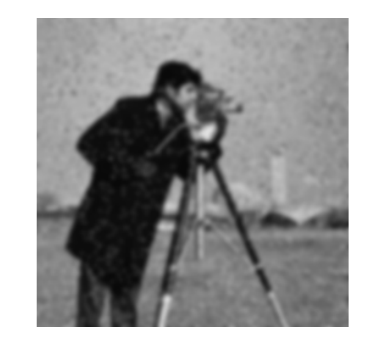
\includegraphics[scale=0.380]{img/visual_perception/camera_man_3.jpeg}
\end{center}
\caption{Camera man image after mean filtering.}
\label{camera_man_3}
\end{figure}

We can see that we have successfully reduced the noise and smooth the image array values in this neighborhood. 
However, it also blurred our image, an inevitable consequence
of these linear filters. This blur can be reduced by tuning the parameters specific to each type of filter.

Equation \ref{simple_filter_equation} can be written as

\begin{equation}
G(u,v) = \frac{1}{(2k+1)^2} \sum_{i=-k}^{k}\sum_{j=-k}^{k} H[i,j]I[u-i, v-j]
\label{simple_filter_equation_2}
\end{equation}

where $\mathbf{H}$ is the weight matrix  called the kernel. We can use $\mathbf{H}$ to add a  weight to every pixel
in the neighborhood.  This generalized form is termed cross-correlation, as it defines a correlation between each pixel and every other pixel in
the neighborhood. For the mean filter defined above, we now represented with the following kernel. A three-by-three matrix filled with the value one-ninth. 

\begin{equation}
\mathbf{H} = \frac{1}{9}\begin{bmatrix}
1 & 1 & 1 \\
1 & 1 & 1 \\
1 & 1 & 1 
\end{bmatrix}
\end{equation}

Another kernel for
noise reduction is the Gaussian kernel, where the center pixel
is weighted more than the neighboring pixels and the weights follow
a Gaussian distribution. 

\begin{equation}
\mathbf{H} = \frac{1}{16}\begin{bmatrix}
1 & 2 & 1 \\
2 & 4 & 2 \\
1 & 2 & 1 
\end{bmatrix}
\end{equation}


Application of a Gaussian kernel in the camera-man image results in Figure \ref{camera_man_4}.  

\begin{figure}[!htb]
\begin{center}
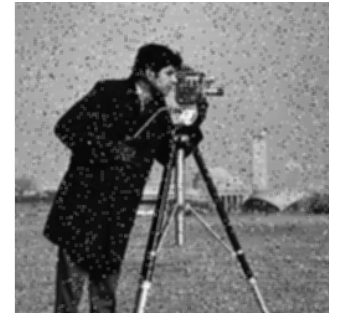
\includegraphics[scale=0.380]{img/visual_perception/camera_man_4.jpeg}
\end{center}
\caption{Camera man image after gaussian filtering.}
\label{camera_man_4}
\end{figure}

\subsection{Convolution Operations}

Now, we will define another useful operation
used for image filtering. A convolution is a cross-correlation, where the filter is
flipped both horizontally and vertically before being
applied to the image. In order to apply the convolution, we take each row of our kernel, flip it and replace it at its corresponding symmetric
position from the middle row. Mathematically, a convolution can be described as
the following equation. Note that we simply manipulated the image coordinates instead
of flipping the kernel. 

What are the advantages of using a convolution over a kernel? Unlike correlation,
convolution is associative, meaning the order of multiplication of
kernels does not matter. We can therefore apply as many consecutive linear kernels
to an image as we want by precomputing
the combined convolution of all the kernels, and then performing
a single convolution of the resulting kernel with the image. As an example, we apply
two linear kernels, $H$ and $F$, by computing $H*F$ and then
applying it to the image. This results in a substantial
reduction in runtime, especially if we need to process images in real-time while
moving in a vehicle. 


\subsection{Applications of Cross-Correlation and Convolution Operations}

Now let's presentsome important applications of cross-correlation and convolution operations. Cross-correlation can be
used for template matching. 

\subsubsection{Template Matching}

Template matching is the problem where we are given a pattern
or a template, and we want to find its location in the image, see \cite{Nazil2013} for an overview. 

\begin{framed}
\begin{remark}{\textbf{Template Matching}}

See the wikipedia entry \url{https://en.wikipedia.org/wiki/Template_matching}. 
See also the OpenCV tutorial on template matching at \url{https://opencv-python-tutroals.readthedocs.io/en/latest/py_tutorials/py_imgproc/py_template_matching/py_template_matching.html}
\end{remark}
\end{framed}

This can be done by finding the location of the highest value of the output
of cross-correlation, between the template and the image. To visualize this better, let's superimpose
the colorized output of cross-correlation on top of our target image. This is shown in Figure \ref{camera_man_5}


\begin{figure}[!htb]
\begin{center}
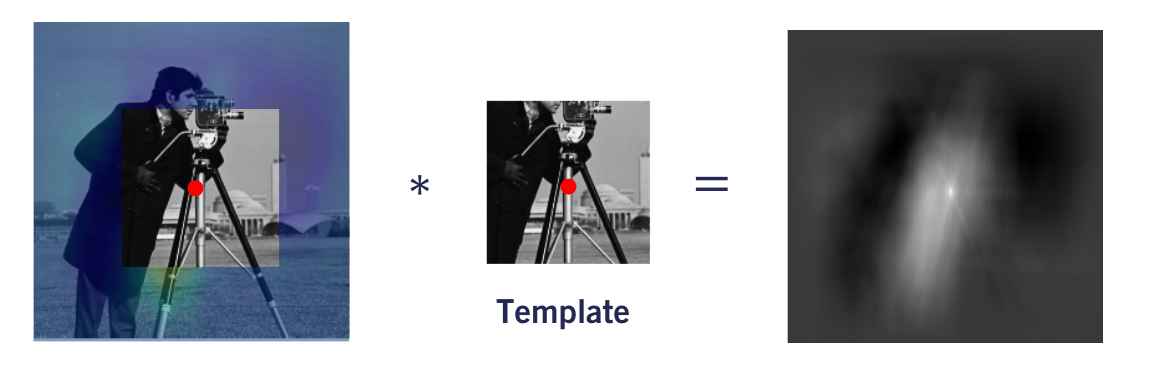
\includegraphics[scale=0.380]{img/visual_perception/camera_man_5.jpeg}
\end{center}
\caption{Template matching.}
\label{camera_man_5}
\end{figure} 


Here red is a high cross-correlation response, while blue is
a very low response. The location of the template
and the image is then the $u, v$ coordinates of the pixel with the highest value from the output of
the cross-correlation. We can check that
our correlation is correct by superimposing
the template on the $u, v$ coordinates we just found. This method can be used as a starting point for
the identification of signs, and even for lean detection, although challenges arise with the approach in practice. 

\subsubsection{Image Gradient Computation}

Another important application that can be performed using convolutions, is image gradient computation. 
This is shown schematically in Figure \ref{camera_man_6}

\begin{figure}[!htb]
\begin{center}
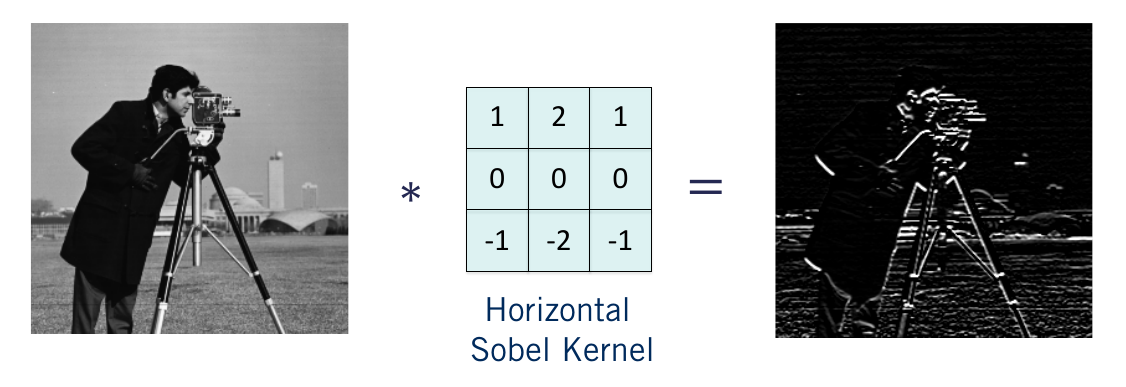
\includegraphics[scale=0.380]{img/visual_perception/camera_man_6.jpeg}
\end{center}
\caption{Schematic of image gradient computation.}
\label{camera_man_6}
\end{figure}

Image gradients can be computed by a convolution with a kernel that performs finite difference. We can rotate our kernel in different orientations
to get vertical, horizontal or even diagonal gradients of an image at a pixel. Image gradients are
extremely useful for the detection of edges and corners, and are used extensively
in self-driving for image feature and object detection, for example. 

\subsection{Summary}

In this section, we discussed how to perform cross-correlation and convolution as well as some of the uses
of these operations. These operations will prove to be very useful later on when we discuss
convolution neural networks. 

\subsection{Questions}

\subsection{Assignements}
